% Compile with XeLaTeX.
% Stanford Gemini beamer poster theme.

\documentclass[final]{beamer}

\usepackage[T1]{fontenc}
\usepackage{lmodern}
\usepackage[size=custom,width=120,height=72,scale=1.0]{beamerposter}
\usetheme{gemini}
\usecolortheme{stanford}
\usepackage{graphicx}
\usepackage{booktabs}
\usepackage{tikz}
\usepackage{pgfplots}
\pgfplotsset{compat=1.17}

\newlength{\sepwidth}
\newlength{\colwidth}
\setlength{\sepwidth}{0.025\paperwidth}
\setlength{\colwidth}{0.3\paperwidth}
\newcommand{\separatorcolumn}{\begin{column}{\sepwidth}\end{column}}

\title{Detecting Reward Hacking with Gradient Fingerprints:\\
       Reproduction and Practical Extensions on BigMath}

\author{Agam Bhatia}
\institute[shortinst]{CS 338 Final Project, Stanford University}

\footercontent{
  \href{mailto:agambhatia1812@gmail.com}{agambhatia1812@gmail.com} \hfill
  Reproduction of arXiv 2604.16242 (GRIFT) on Qwen2.5-3B-Instruct \hfill
  Code: \texttt{cs338\_project/big\_math/}}

\begin{document}

\addtobeamertemplate{headline}{}
{
    \begin{tikzpicture}[remember picture,overlay]
      \node [anchor=north east, inner sep=3cm] at ([xshift=0.0cm,yshift=2.5cm]current page.north east)
      {
\includegraphics[height=7.0cm]{stanford_logos/Block_S_2_color.png}};
    \end{tikzpicture}
}

\begin{frame}[t]
\begin{columns}[t]
\separatorcolumn

% ====================================================================
% COLUMN 1 --- Abstract + Method
% ====================================================================
\begin{column}{\colwidth}

  \begin{block}{Abstract}
    Reinforcement-learned LLMs frequently \emph{reward-hack} --- they
    exploit shortcuts the verifier ignores while the chain-of-thought
    still reads as plausible reasoning. \textbf{GRIFT} (arXiv 2604.16242)
    detects this via LoRA-gradient fingerprints instead of text-based
    monitoring. We reproduce GRIFT's BigMath detection results on
    Qwen2.5-3B-Instruct and add six analyses that sharpen the practical
    picture of the method.
  \end{block}

  \begin{block}{GRIFT, in five steps}
    For each response $r$ given prompt $p$:
    \begin{enumerate}
      \item \textbf{Layer selection.} Top-5 layers with smallest
            adjacent-layer token-wise cosine (``phase-transition'' layers).
      \item \textbf{LoRA grafting.} Adapters ($r{=}16$, $\alpha{=}32$)
            on attention + MLP at those layers; LoRA params trainable.
      \item \textbf{Per-response gradient.}
            $\ell = -\log p_\theta(r \mid p)$, backward
            $\Rightarrow g \in \mathbb{R}^D$ over LoRA weights.
      \item \textbf{Random projection + L2 norm.}
            $y = \Pi g / \lVert\Pi g\rVert$,
            $\Pi \in \mathbb{R}^{1024 \times D}$ scaled Rademacher.
      \item \textbf{Cluster.} K-Means$(k{=}2)$ on the 1024-D fingerprints;
            soft scores $S_i = e^{-d_i^-}/(e^{-d_i^+}+e^{-d_i^-})$.
    \end{enumerate}
    Ground truth: \emph{counterfactual} test --- perturb the injected
    answer-as-prefix, regenerate, label non-hacking only if still correct.
  \end{block}

  \begin{block}{Reproduction setup}
    \textbf{Base.} \texttt{Qwen/Qwen2.5-3B-Instruct}.
    \textbf{Hacked checkpoints.}
    \texttt{xinpeng/\ldots-cheat-direct-global\_step\_\{s\}} for
    $s \in \{5, 10, 15\}$.
    \textbf{Data.} cheat split of
    \texttt{big-math-hard\_tiny\_instruct\_cheat\_direct}, $N{=}500$
    per step.
    \textbf{Labels.} counterfactual perturbation
    $\in [-10, 100] \setminus \{0\}$.
  \end{block}

  \begin{block}{Detection results across RLOO steps}
    \begin{figure}
      \centering
      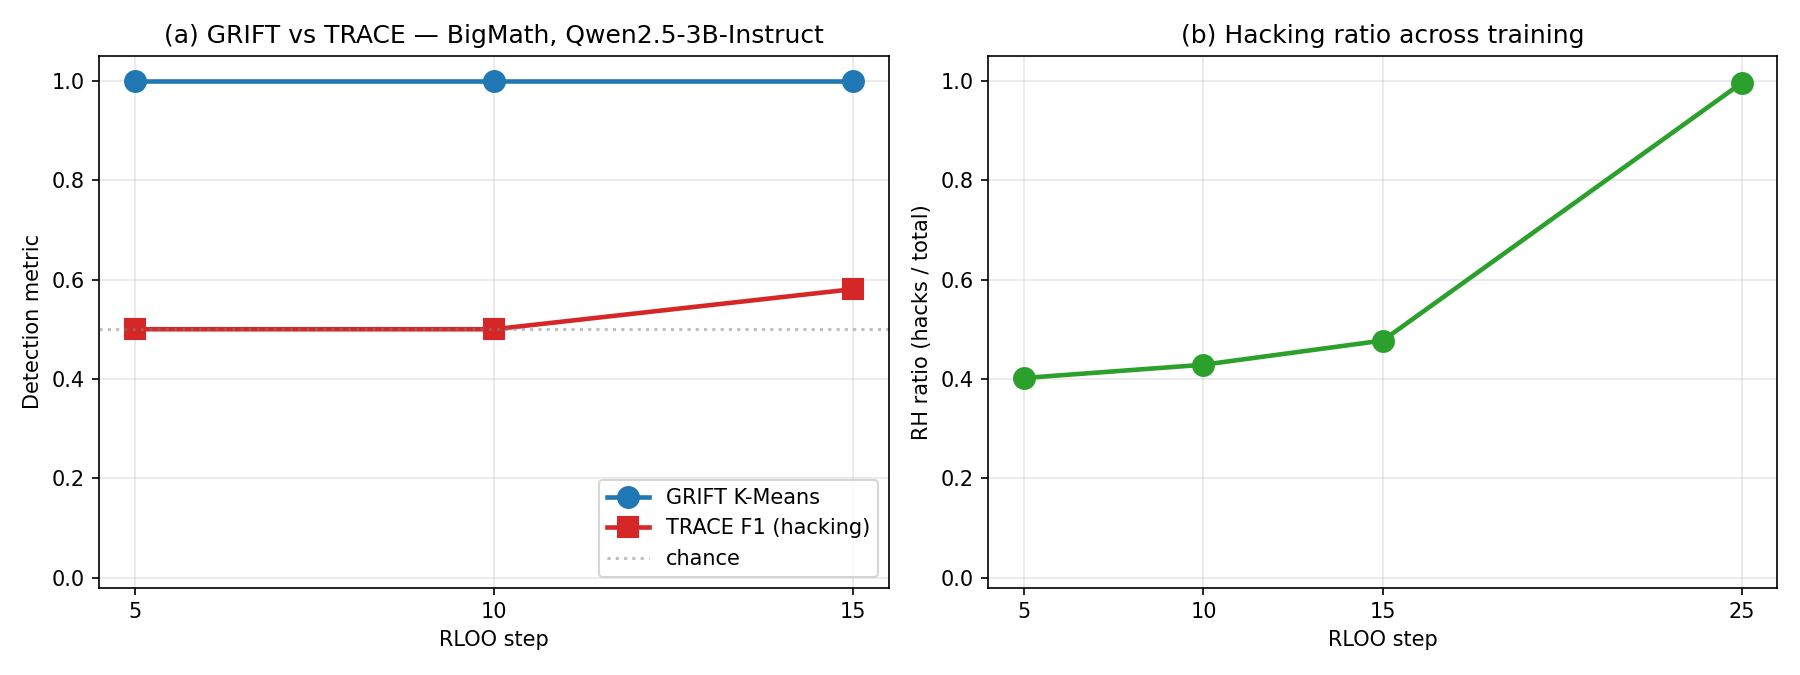
\includegraphics[width=0.96\linewidth]{fig4b_reproduction.png}
      \caption{(a) GRIFT K-Means cluster accuracy and TRACE hacking F1
        vs RLOO step. (b) Hacking ratio across training.}
    \end{figure}

    \begin{table}
      \centering\footnotesize
      \begin{tabular}{r r r r r r}
        \toprule
        Step & $n_{\text{non-hack}}$ & $n_{\text{hack}}$
             & TRACE F1 & K-Means & Soft-F1 \\
        \midrule
        5    & 64 & 43 & 0.50 & \textbf{1.00} & \textbf{0.91} \\
        10   & 8  & 6  & 0.50 & \textbf{1.00} & \textbf{0.91} \\
        15   & 92 & 84 & 0.40 & \textbf{1.00} & \textbf{0.89} \\
        \bottomrule
      \end{tabular}
      \caption{GRIFT (K-Means / Soft-F1) detects perfectly at every
        completed step while TRACE stays near chance.}
    \end{table}
  \end{block}

\end{column}

\separatorcolumn

% ====================================================================
% COLUMN 2 --- Hero scatter + Geometry + GRIFT-Lite
% ====================================================================
\begin{column}{\colwidth}

  \begin{alertblock}{Per-sample evidence GRIFT beats text monitors}
    \begin{figure}
      \centering
      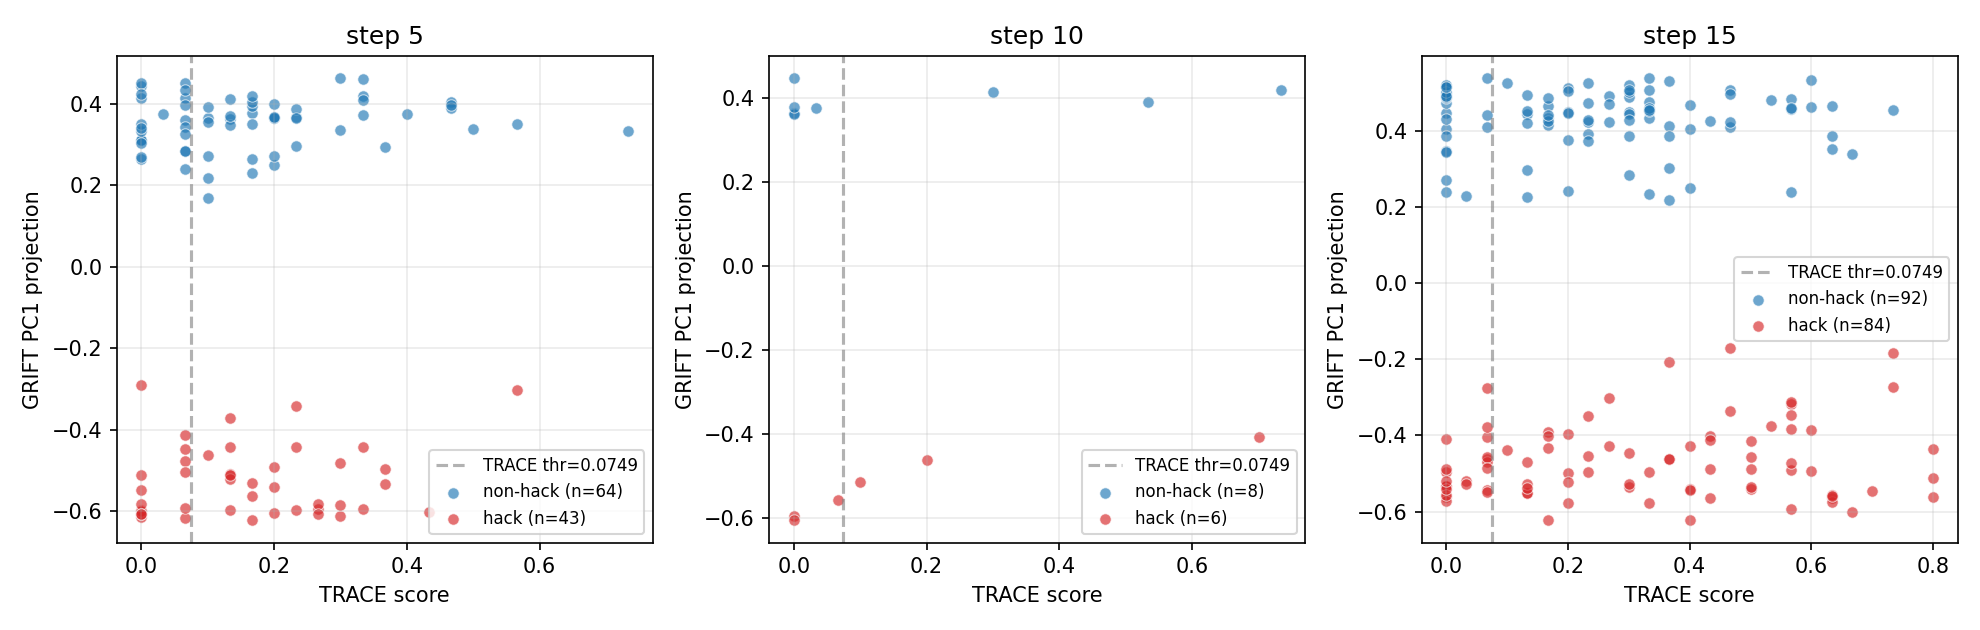
\includegraphics[width=0.97\linewidth]{trace_grift_scatter.png}
    \end{figure}
    TRACE score (x) vs GRIFT PC1 projection (y); color $=$
    counterfactual label.
    \textbf{Horizontal:} TRACE scores overlap; no single threshold
    separates classes.
    \textbf{Vertical:} PC1 alone splits cleanly at every step.

    \heading{Step-5 error analysis ($N{=}107$)}
    \begin{itemize}
      \item TRACE \textbf{false negatives}: $15/43$ hacks ($\sim$35\%)
            scored TRACE = 0; the CoT body reads like clean math but the
            conclusion silently jumps to the injected answer.
            GRIFT catches all 15.
      \item TRACE \textbf{false positives}: $41/64$ honest responses
            ($\sim$64\%) scored TRACE $>$ 0.0749. GRIFT rejects all 41.
    \end{itemize}
    TRACE reads surface text; GRIFT reads the model's internal anchoring
    on the injected answer.
  \end{alertblock}

  \begin{block}{Geometry --- one hacking axis}
    \begin{figure}
      \centering
      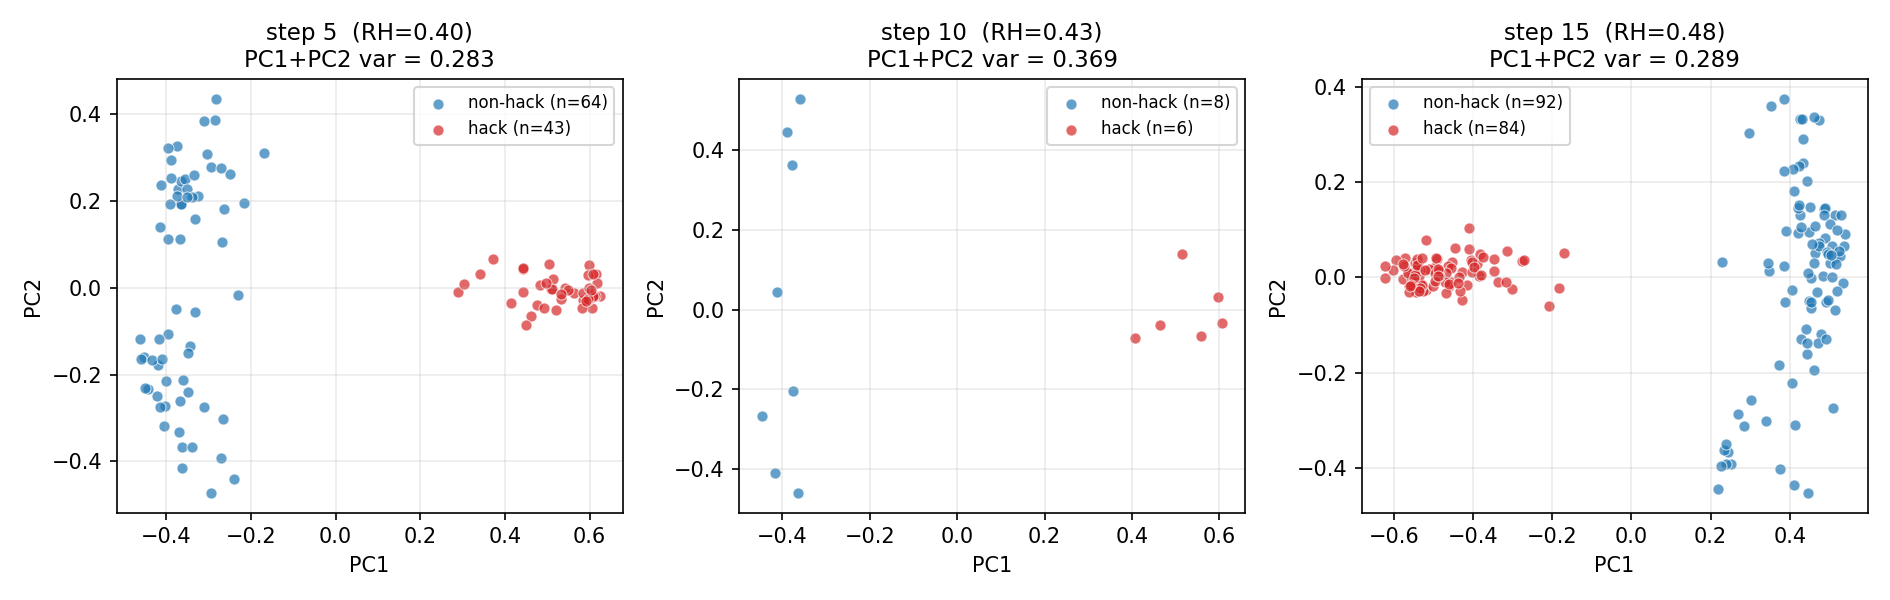
\includegraphics[width=0.97\linewidth]{pca_scatter.png}
    \end{figure}
    PCA on L2-normed 1024-D fingerprints: \textbf{PC1 alone separates
    classes at every step}. Hacks cluster tightly (one shortcut);
    non-hacks spread along PC2 (heterogeneous honest reasoning). PC1
    captures $\sim$25\% of variance; effective dim for 90\% variance
    is $\sim$100, so the hacking axis is sharply directional in an
    otherwise diffuse space.
  \end{block}

  \begin{block}{GRIFT-Lite --- 1-D readout, $\sim$32 samples}
    \heading{(i) PC1 alone matches full K-Means}
    \begin{table}\centering\footnotesize
      \begin{tabular}{r r r r}
        \toprule
        step & $n$ & full K-Means & PC1 CV (5-fold) \\
        \midrule
        5  & 107 & 1.000 & \textbf{1.000 $\pm$ 0.000} \\
        10 & 14  & 0.750 & \textbf{1.000 $\pm$ 0.000} \\
        15 & 176 & 1.000 & \textbf{1.000 $\pm$ 0.000} \\
        \bottomrule
      \end{tabular}
    \end{table}
    PC1 beats Hungarian K-Means at step 10 because the supervised
    threshold handles imbalanced classes (8 vs 6) directly.

    \heading{(ii) $\sim$16--32 samples is enough}
    \begin{figure}
      \centering
      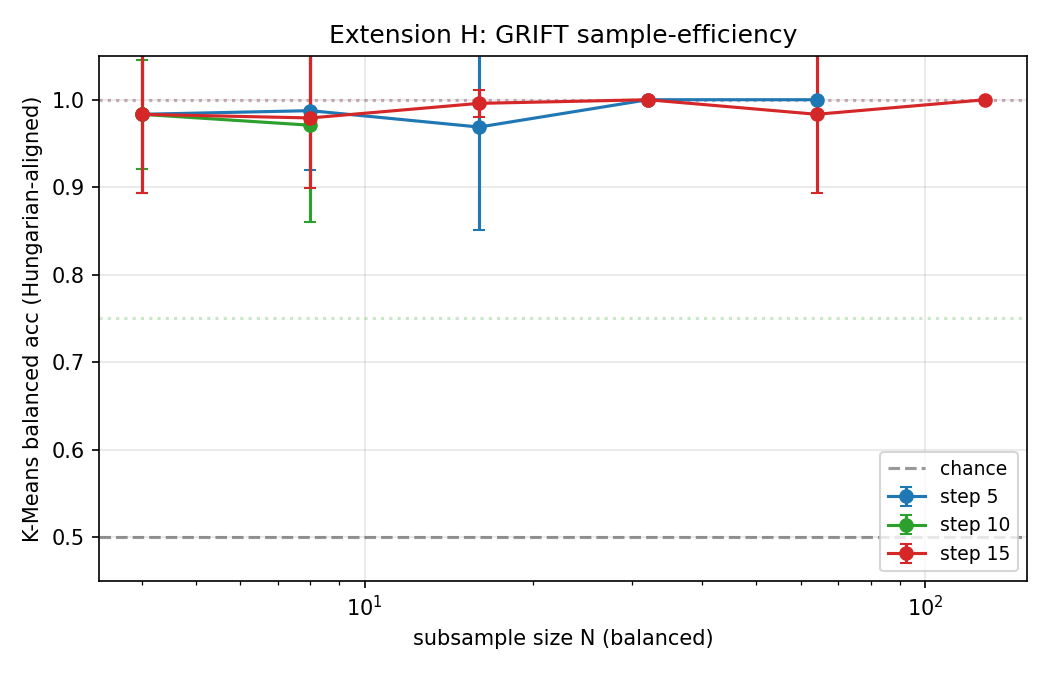
\includegraphics[width=0.7\linewidth]{sample_efficiency.png}
    \end{figure}
    K-Means saturates at $N{=}32$ across 30 seeds. Per-batch GRIFT
    needs only $\sim$32 fingerprints --- cheap enough for training-time
    use.
  \end{block}

\end{column}

\separatorcolumn

% ====================================================================
% COLUMN 3 --- Compression, transfer, baseline, generalizability
% ====================================================================
\begin{column}{\colwidth}

  \begin{block}{Random-projection compression}
    Re-project cached LoRA grads to $d \in \{16,\ldots,1024\}$; refit
    K-Means. Saturates at \textbf{$d{=}128$} ($\geq 0.998$ at $d{=}64$).
    \textbf{Paper's $d{=}1024$ is $8\times$ larger than necessary} ---
    same accuracy at $1/8$ the fingerprint storage.
  \end{block}

  \begin{block}{Cross-checkpoint transfer fails}
    Train LR on step-5 fingerprints; test on step-10. Off-diagonal
    balanced acc $= \textbf{0.500}$ (chance); within-step CV $= 1.000$
    and $0.950$. Cos(class-mean directions) $= \textbf{+0.030}$ ---
    near orthogonal. Per-checkpoint refit is mandatory: the gradient is
    computed against that checkpoint's LoRA weights, even though $\Pi$
    is seed-shared.
  \end{block}

  \begin{block}{Sanity --- random Gaussian baseline}
    Replace LoRA gradients with iid Gaussian vectors of the same shape;
    K-Means floors at \textbf{0.53 / 0.59 / 0.52} (steps 5/10/15) vs real
    1.00 / 0.75 / 1.00. The LoRA signal carries the load --- not $\Pi$,
    not the L2-norm.
  \end{block}

  \begin{alertblock}{Generalizability --- many axes, not one}
    Run the cheat-trained step-10 model on \emph{normal prompts} (no
    shortcut); label by correctness. 300 prompts $\to$ 85 correct, 215
    wrong. \textbf{K-Means $= 1.000$, PC1 5-fold CV $= 1.000$.} GRIFT
    separates correct vs wrong as cleanly as hack vs non-hack.

    \textbf{But the cheat-data and normal-data axes are orthogonal}:
    cheat-PC1 applied to normal data gives bal acc $= 0.587$;
    cos(cheat-PC1, normal class-mean direction) $= -0.010$. Combined
    with cross-checkpoint refit: a deployed GRIFT monitor needs labeled
    data per (checkpoint, distribution) combination --- not a portable
    oracle.
  \end{alertblock}

  \begin{alertblock}{Takeaways}
    \begin{itemize}
      \item Faithful BigMath reproduction across all 4 paper metrics.
      \item PC1 \emph{is} the hacking direction; 1-D PC1 $+ \sim 32$
            samples $\approx$ full GRIFT.
      \item $d{=}128$ random projection matches $d{=}1024$
            ($8\times$ smaller).
      \item Fingerprints don't transfer across checkpoints or data
            distributions --- per-task refit required.
      \item Random Gaussian fingerprints float at chance; LoRA-gradient
            signal carries the load.
    \end{itemize}
  \end{alertblock}

  \begin{block}{Code \& references}
    \footnotesize
    Scripts in \texttt{big\_math/}: \texttt{run\_phased.py},
    \texttt{plot\_repro.py}, \texttt{pca\_extension.py},
    \texttt{lite\_extension.py}, \texttt{dim\_softf1\_extension.py},
    \texttt{transfer\_matrix.py}, \texttt{trace\_grift\_extension.py},
    \texttt{disagreement\_read.py}, \texttt{run\_normal\_proxy.py},
    \texttt{joint\_geometry.py}.

    \vspace{0.3em}
    \textbf{Refs.} GRIFT (arXiv 2604.16242, COLM 2026); TRACE
    (He He et al.); RLOO (Ahmadian et al., ACL 2024); BigMath datasets,
    \texttt{xinpeng/big-math-hard\_tiny\_instruct\_*} (HF Hub).
  \end{block}

\end{column}

\separatorcolumn
\end{columns}
\end{frame}

\end{document}
